\documentclass[12pt]{report}


% All macros

%  First find out if we're running pdftex
\usepackage{ifpdf}

\ifpdf
\pdfcompresslevel 5
\fi

% Times is nicer with pdf
\usepackage{times}
% American style
\usepackage[american]{babel}

\usepackage[T1]{fontenc}

% To make typesetting easier
\usepackage{xspace}

% Generate an index
\usepackage{makeidx}
\makeindex

% Some convenient macros:
%  Add text to index and print it also
\newcommand{\textindex}[1]{#1\index{#1}\xspace}
% Add text to index and print it also with \code{}
\newcommand{\codeindex}[1]{\code{#1}\index{#1@\texttt{#1}}\xspace}
% A version without xspace - I had some strange problems with commas
% afterwards.
\newcommand{\codeindexwo}[1]{\texttt{#1}\index{#1@\texttt{#1}}}

% Control placement of floats
%\usepackage{here}
\usepackage{float}

% Version number of document - increment occasionally ;-)
\newcommand{\version}{1.0}

% Print a footer everywhere with current date
% prelim2e needs \thistime
\newcount\hours
\newcount\minutes
\def\SetTime{\hours=\time
        \global\divide\hours by 60
        \minutes=\hours
        \multiply\minutes by 60
        \advance\minutes by-\time
        \global\multiply\minutes by-1 }
\SetTime
\def\thistime{\number\hours:\ifnum\minutes<10 0\fi\number\minutes}
\usepackage[time]{prelim2e}
\renewcommand{\PrelimWords}{RIVER ABI \version}

% Some commands:
\newcommand{\editornote}[1]{\footnote{#1}}

%Typesetting of registers
\newcommand{\reg}[1]{{\texttt{\%#1}}\xspace}
\newcommand{\RAX}{\reg{rax}}
\newcommand{\RBX}{\reg{rbx}}
\newcommand{\RCX}{\reg{rcx}}
\newcommand{\RDX}{\reg{rdx}}
\newcommand{\RSI}{\reg{rsi}}
\newcommand{\RDI}{\reg{rdi}}
\newcommand{\RBP}{\reg{rbp}}
\newcommand{\RSP}{\reg{rsp}}
\newcommand{\RIP}{\reg{rip}}

%Typesetting of opcodes
\newcommand{\op}[1]{\texttt{#1}}

%Typesetting common names
\newcommand{\MMX}{\emph{MMX}\xspace}
\newcommand{\xARCH}{AMD64\xspace}
\newcommand{\threednow}{3DNow!\xspace}

% Typesetting paths and files
\newcommand{\path}[1]{\texttt{#1}\xspace}

% Typesetting program code
\newcommand{\code}[1]{\texttt{#1}\xspace}

% Long Hrule
\newcommand{\Hrule}{\noindent\rule{\linewidth}{0.3mm}}

\usepackage{xcolor}
% Use Hyperref for PDF support - this should be last
\ifpdf
\usepackage[pdftex,colorlinks,linkcolor={blue!50!black}]{hyperref}
\usepackage{changebar}
\else
\usepackage[dvips,colorlinks,linkcolor={blue!50!black}]{hyperref}
\usepackage{changebar}
\fi

% Make `_' an ordinary character.
\catcode`_=12

% The Intel386 psABI document.
\newcommand{\intelabi}{Intel386 ABI\xspace}

\newcommand{\byte}{byte\xspace}
\newcommand{\twobyte}{twobyte\xspace}
\newcommand{\fourbyte}{fourbyte\xspace}
\newcommand{\eightbyte}{eightbyte\xspace}
\newcommand{\eightbytes}{eightbytes\xspace}
\newcommand{\sixteenbyte}{sixteenbyte\xspace}

\newcommand*{\cbnew}{\marginpar{\textsf{New}}}

\newcommand{\myfontsize}{\fontsize{9}{10}\selectfont}

\usepackage{listings}
\usepackage{multirow, multicol}

%%% Local Variables:
%%% mode: latex
%%% TeX-master: "abi"
%%% End:


\begin{document}

\author{Edited by\\
  Teodor Stoenescu\thanks{tstoenescu@bitdefender.com},
  Alexandra Sandulescu\thanks{asandulescu@bitdefender.com}}

\title{River Application Binary Interface\\
Version \version}
\maketitle
\tableofcontents
%%\listoftables
%%\listoffigures

\section*{Revision History}

\begin{description}
	\item[1.0][09.02.2018] Document rep prefix instrumentation \autoref{}.
\item[0.3][28.01.2016] Added \autoref{} detailing instruction reassembly.
\item[0.2][26.01.2016] Added chapter detailing the binary translation - \autoref{}.
Added several new meta instructions - \autoref{}.
Added the track instruction family.
Substituted chapter numbers with cross references.
\item[0.1][09.09.2015] Renamed symbop instruction set to track and pretrack.
Covers the pretrack instruction set.
Added individual flag tracking.
Added a brief description of the current API.
\item[0.0][20.07.2015] Initial release. Covers general instruction layout as well as the river instruction set.
\end{description}

\chapter{River internal instruction representation}
Since this documentation is subject to change please consult the river.h header file for an updated version.\\
Instructions are represented in the river intermediate representation as fixed length structures as defined below. This comes in handy since most translators work on arrays of instructions.

\lstinputlisting[language=C]{../cheatsheet/code/RiverInstruction.h}

Modifiers are described in \autoref{sec:modifiers}, specifiers in \autoref{sec:specifiers}, family in \autoref{sec:instrfamilies}. OpTypes are documented in \autoref{sec:operands-and-operand-types} along with operands.

\section{Modifiers}
\label{sec:modifiers}
Instruction modifiers are optional instruction features introduced by x86 instruction prefixes.\\
\begin{tabular}[t]{| p{6cm} | p{10cm} |}
\hline
	\textbf{Modifier name} & \textbf{Modifier meaning}\\ \hline
	RIVER\_MODIFIER\_NOSEG & Default modifier, used as a placeholder when no other modifiers are specified.\\ \hline
	RIVER\_MODIFIER\_ESSEG & \multirow{6}{*}{The instruction has been prefixed with a segment selector.} \\
	RIVER\_MODIFIER\_CSSEG &\\
	RIVER\_MODIFIER\_SSSEG &\\
	RIVER\_MODIFIER\_DSSEG &\\
	RIVER\_MODIFIER\_FSSEG &\\
	RIVER\_MODIFIER\_GSSEG &\\ \hline
	RIVER\_MODIFIER\_EXT & The instruction has a two byte opcode. (0x0F is the first byte)\\ \hline
	RIVER\_MODIFIER\_O8 & (No corresponding prefix) The instruction operates on 8 bit operands.\\ \hline
	RIVER\_MODIFIER\_O16 & The instruction operates on 16 bit operands.\\ \hline
	RIVER\_MODIFIER\_A16 & The instruction uses 16 bit addressing mode.\\ \hline
	RIVER\_MODIFIER\_LOCK & The instruction has a LOCK prefix.\\ \hline
	RIVER\_MODIFIER\_REP & \multirow{3}{*}{The instruction has a REP/REPZ/REPNZ prefix.}\\
	RIVER\_MODIFIER\_REPZ &\\
	RIVER\_MODIFIER\_REPNZ &\\ \hline
\end{tabular}

\section{Specifiers}
\label{sec:specifiers}
Instruction specifiers are decorations introduced by the disassembler in order to aid data flow analysis.\\
\begin{tabular}[t]{| p{6cm} | p{10cm} |}
\hline
	\textbf{Specifier name} & \textbf{Specifier meaning}\\ \hline
	RIVER\_SPEC\_MODIFIES\_OP(x) & \multirow{5}{10cm}{The current instruction modifies the specified operand. NOTE: Keep in mind that RIVER_SPEC_MODIFIES_OP1 actually corresponds to RIVER_SPEC_MODIFIES_OP(0).}\\
	RIVER\_SPEC\_MODIFIES\_OP1 &\\
	RIVER\_SPEC\_MODIFIES\_OP2 &\\
	RIVER\_SPEC\_MODIFIES\_OP3 &\\
	RIVER\_SPEC\_MODIFIES\_OP4 &\\ \hline
	RIVER\_SPEC\_MODIFIES\_FLG & The instruction modifies at least one CPU flag. (This specifier might be deprecated in the future and replaced with individual per-flag versions)\\ \hline
	RIVER\_SPEC\_IGNORES\_OP(idx) & \multirow{5}{10cm}{Used in combination with RIVER\_SPEC\_MODIFIES\_OP(x), specifies that the current operand is only used as an output operand. NOTE: Keep in mind that RIVER\_SPEC\_IGNORES\_OP1 actually corresponds to RIVER\_SPEC\_IGNORES\_OP(0).} \\
	RIVER\_SPEC\_IGNORES\_OP1 &\\
	RIVER\_SPEC\_IGNORES\_OP2 &\\
	RIVER\_SPEC\_IGNORES\_OP3 &\\
	RIVER\_SPEC\_IGNORES\_OP4 &\\ \hline
	RIVER\_SPEC\_IGNORES\_FLG & The instruction ignores all CPU flags. (To be deprecated soon).\\ \hline
\end{tabular}

\section{Instruction families}
\label{sec:instrfamilies}
Instruction families are the core of the river design. \autoref{chapter:instrfamiliesabi} gives a more detailed analysis of the available families.\\
\begin{tabular}{| p{6cm} | p{10cm} |}
\hline
	\textbf{Family name} & \textbf{Family meaning}\\ \hline
	RIVER_FAMILY_NATIVE & Native instructions produced by the x86 disassembler.\\ \hline
	RIVER_FAMILY_PRETRACK & Instruction family that handles symbolic variable tracking. These instructions are inserted directly into the original instruction stream.\\ \hline
	RIVER_FAMILY_TRACK & Instruction family that handles symbolic variable tracking. These instructions are inserted in a separate instruction stream.\\ \hline
	RIVER_FAMILY_PREMETA & Instruction produced by the disassembler that further specify the following native instruction.\\ \hline
	RIVER_FAMILY_POSTMETA & Instruction produced by the disassembler that further specify the previous native instruction.\\ \hline
	RIVER_FAMILY_RIVER & Instruction family that enables reversible code.\\ \hline
\end{tabular} \\
\newline
Furthermore some instruction families may be further decorated with the following flags.\\
\begin{tabular}{| p{8cm} | p{8cm} |}
\hline
	\textbf{Family name} & \textbf{Family meaning}\\ \hline
	RIVER_FAMILY_FLAG_IGNORE & The current instruction has been marked for lazy deletion.\\ \hline
	RIVER_FAMILY_FLAG_ORIG_xSP & The current instruction needs access to the native stack pointer.\\ \hline
	RIVER_FAMILY_FLAG_METAPROCESSED & The current instruction has been completely split up in metaoperations.\\ \hline
\end{tabular}

\section{Operands and operand types}
\label{sec:operands-and-operand-types}
The opTypes field endcodes the operand type while the operands field encodes the actual operand. The opTypes field can have the following base values.\\
\begin{tabular}[t]{| p{6cm} | p{10cm} |}
\hline
	\textbf{Operand type} & \textbf{Meaning}\\
	RIVER_OPTYPE_NONE & This type specifies that the current operand is not used.\\ \hline
	RIVER_OPTYPE_IMM & The current operand is an immediate value.\\ \hline
	RIVER_OPTYPE_REG & The current operand is a CPU register.\\ \hline
	RIVER_OPTYPE_MEM & The current operand is an address.\\ \hline
\end{tabular}\\
\newline
Furthermore the basic operand types can be combined with one of the following size specifiers.\\
\begin{tabular}[t]{| p{6cm} | p{10cm} |}
	\hline
	\textbf{Operand size} & \textbf{Meaning}\\ \hline
	RIVER_OPSIZE_32 & 32-bit operand. (This is the default value)\\ \hline
	RIVER_OPSIZE_16 & 16-bit operand.\\ \hline
	RIVER_OPSIZE_8 & 8-bit operand.\\ \hline
\end{tabular}\\
\newline
Last but not least the operand type can have the RIVER_OPFLAG_IMPLICIT flag set in order to distinguish between explicit operands and operands implicitly added by the disassembler.\\
\newline
The RiverOperand union encapsulates all possible operand configurations and is described in the following chapters.\\

\subsection{Immediate operands}
\label{ssec:immediate-operands}
Depending on the operand size immediate values are stored in the RiverOperand::asImm8, RiverOperand::asImm16 or RiverOperand::asImm32 members.\\
\subsection{Register operands}
\label{ssec:register-operands}
Register operands are stored in the RiverOperand::asRegister member. This is a 32-bit field where the least significant eight bits encode the register name, while the remaining bits are used for register versioning (in order to achieve SSA at a basic block level). Register name encoding is divided between general purpose and other registers.\\
\newline
The general purpose registers can be specified by combining the register name with the register size as described in the table below.\\
\begin{tabular}{| p{3.6cm} | p{3.2cm} | p{1cm} | p{1cm} | p{1cm} | p{1cm} | p{1cm} | p{1cm} | p{1cm} |}
\hline
& RIVER_REG_xAX & *_xCX & *_xDX & *_xBX & *_xSP & *_xBP & *_xSI & *_xDI\\ \hline
RIVER_REG_SZ32 & EAX & ECX & EDX & EBX & ESP & EBP & ESI & EDI\\ \hline
RIVER_REG_SZ16 & AX & CX & DX & BX & SP & BP & SI & DI\\ \hline
RIVER_REG_SZ8_L & AL & CL & DL & BL & - & - & - & -\\ \hline
RIVER_REG_SZ8_H & AH & CH & DH & BH & - & - & - & -\\ \hline
\end{tabular}\\
\newline
Other registers have individual register notations.\\
\begin{tabular}{| p{5cm} | p{5cm} | p{5cm} |}
	\hline
	\textbf{Segment registers} & \textbf{Control registers} & \textbf{Debug registers} \\ \hline
	RIVER_REG_ES RIVER_REG_CS RIVER_REG_SS RIVER_REG_DS RIVER_REG_FS RIVER_REG_GS &
	RIVER_REG_CR0 RIVER_REG_CR2 RIVER_REG_CR3 RIVER_REG_CR4 &
	RIVER_REG_DR0 RIVER_REG_DR1 RIVER_REG_DR2 RIVER_REG_DR3 RIVER_REG_DR4 RIVER_REG_DR5 RIVER_REG_DR6 RIVER_REG_DR7\\ \hline
\end{tabular}\\

\subsection{Address operands}
\label{ssec:address-operands}
Address operands are stored as a pointer to a structure containing following fields.\\
\begin{tabular}{| p{6cm} | p{10cm} |}
	\hline
	\textbf{RiverAddress field name} & \textbf{Meaning}\\ \hline
	type & Encodes valid address fields as described below.\\ \hline
	base & Encodes the base register. Valid only if type has the RIVER_ADDR_BASE flag set.\\ \hline
	index & Encodes the index register. Valid only if type has the RIVER_ADDR_INDEX flag set.\\ \hline
	disp.d8 & Encodes a 8-bit displacement. Valid only if type has the RIVER_ADDR_DISP8 flag set.\\ \hline
	disp.d32 & Encodes a 32-bit displacement. Valid only if type has the RIVER_ADDR_DISP flag set. (Mutually exclusive with disp.d8)\\ \hline
	scaleAndSegment & Encodes the address scale and segment in a single byte. Use the provided getters and setters for convenient access. The scale is only valid if type has the RIVER_ADDR_SCALE flag set.\\ \hline
\end{tabular}\\
\newline
As a short reminder the x86 addressing works by evaluating the following expression:\\
\[address = base + scale * index + displacement\]
Where:
\begin{itemize}
	\item any of the aforementioned components are optional
	\item the scale can have values of 1,2,4 and 8
	\item the displacement can be 8 or 32 bits
\end{itemize}

\section{Unused registers}
\label{sec:unused-register}
The RiverInstruction contains a unusedRegisters member. The disassembler marks all the general purpose registers unaffected by the current instruction. This comes in handy while reassembling.\\
\newline
For instance, non-native instructions make use of a modified stack pointer register (ESP). When these instructions need access to the original ESP (RIVER_FAMILY_ORIG_xSP is set) some form of register reallocation needs to be performed. The assembler makes use of one of the unused registers to hold the original ESP value.\\

\chapter{Instruction families ABI}
\label{chapter:instruction-families-abi}
\section{Native family ABI}
\label{sec:native-family-abi}
Detailing the x86 instruction set is beyond the scope of this document. Check out \footnote{Intel 64 and IA-32 Architectures Software Developer Manual \url{https://www.intel.com/content/dam/www/public/us/en/documents/manuals/64-ia-32-architectures-software-developer-manual-325462.pdf}} for an in depth explanation.\\
\newline
Furthermore, \footnote{X86 Opcode and Instruction Reference \url{http://ref.x86asm.net/coder32.html}} has a really good overview of the whole instruction set.\\

\section{River family ABI}
\label{sec:river-family-abi}
The river instruction family handles code reversibility by saving values that are about to be destroyed in an execution log. Reversing code execution simply translates to restoring the initial values. Following instructions are available:\\
\begin{tabular}{| l | l | l |}
	\hline
	\textbf{Instruction mnemonic} & \textbf{Opcode} & \textbf{Meaning} \\ \hline
	riverpushf & 0x9C & Save the EFLAGS register.\\ \hline
	riverpopf & 0x9D & Restore the EFLAGS register.\\ \hline
	riverpush reg & 0x50 + r & Save a general purpose register.\\ \hline
	riverpop reg & 0x58 + r & Restore a general purpose register.\\ \hline
	riverpush mem & 0xFF /6 & Save a memory location.\\ \hline
	riverpop mem & 0x8F & Restore a memory location.\\ \hline
\end{tabular}\\
While reassembling, the river instructions are converted into their native counterparts.\\
\newline
The river instruction set needs a separate ESP register. Transitioning to and from a river instruction is achieved using a single xchg instruction. Below are two examples. The second example also shows how the register renaming works.\\
\newline
\begin{tabular}{| l | l |}
	\hline
	\textbf{Original code} & \textbf{Reassembled code}\\ \hline
	\multirow{3}{*}{riverpush [eax+4*ecx]} & xchg esp, [espSave]\\
    & push [eax+4*ecx]\\
	& xchg esp, [espSave]\\ \hline
	\multirow{5}{*}{riverpush esp} & xchg esp, [espSave]\\
	& xchg eax, esp\\
	& push eax\\
	& xchg eax, esp\\
	& xchg esp, [espSave]\\ \hline
\end{tabular}\\

\section{Meta family ABI (both pre- and postmeta)}
\label{sec:meta-family-abi}
Meta instructions are generated by the disassembler in order to add further detail to the native instruction family. There are two instructions available in the meta instruction family.\\
\newline
\begin{tabular}{| l | l | l |}
	\hline
	\textbf{Instruction mnemonic} & \textbf{Opcode} & \textbf{Meaning}\\ \hline
	metaadd reg, imm8 & 0x83 /0 & Add an immediate value to a register. No flags are altered.\\ \hline
	metasub reg, imm8 & 0x83 /5 & Subtract an immediate value to a register. No flags are altered.\\ \hline
	metamov reg, mem & 0x8B & Move memory to register (32 bit).\\ \hline
	metamov mem, reg & 0x89 & Move register to memory (32 bit).\\ \hline
	metamov mem, imm32 & 0xC7 & Move immediate value to memory.\\ \hline
	metamov mem1, mem2 & 0xA5 & Copy 4 bytes from mem2 to mem1.\\ \hline
\end{tabular}

\section{Pretrack family ABI}
\label{sec:pretrack-family-abi}
Pretrack instructions handle the saving of immediate values in order to correctly track symbolic expressions. Similar to the river instructions, pretrack instructions require a separate shadow stack.\\
\newline
\begin{tabular}{| l | l | l |}
	\hline
	\textbf{Instruction mnemonic} & \textbf{Opcode} & \textbf{Meaning}\\ \hline
	pretrackpushf & 0x9C & Save a copy of the flags register.\\ \hline
	pretrackpush reg & 0x50 + r & Save the value of the register.\\ \hline
	pretracklea mem & 0x8D & Save the address specified as the first operand.\\ \hline
	pretrackpush mem & 0xFF /6 & Save the content at the specified address.\\ \hline
\end{tabular}\\
\newline
While reassembling pretrack instructions are converted into their native counterparts. Transitioning to the pretrack family requires an extra xchg instruction.\\
\newline
Specifically, the pretracklea instruction requires an additional register. The assembler picks an unused register dynamically. Below is an example of said behavior.\\
\newline
\begin{tabular}{| l | l |}
	\hline
	\textbf{Original code} & \textbf{Reassembled code}\\ \hline
	\multirow{6}{*}{pretracklea [eax+4*ecx]} & xchg esp, [espSave]\\
	& mov [tmp], edx\\
	& lea edx, [eax+4*ecx]\\
	& push edx\\
	& mov edx, [tmp]\\
	& xchg esp, [espSave]\\ \hline
\end{tabular}

\section{Track family ABI}
\label{sec:track-family-abi}
\begin{tabular}{| l | l | p{10cm} |}
	\hline
	\textbf{Instruction mnemonic} &	\textbf{Opcode} & \textbf{Meaning}\\ \hline
	trackinit & 0xB8 & Initialize the tracking register. Corresponds to \textit{mov edi, 0}.\\ \hline
	trackclean imm8 & 0xC3 & Marks the end of tracking for the current instruction. Corresponds to \textit{retn}.\\ \hline
	trackflags imm8 & 0x8D & Select which flags are used as input. Corresponds to \textit{pushf}.\\ \hline
	markflags imm8 & 0x9D & Selects which flags are used as output. Corresponds to \textit{popf}.\\ \hline
	trackreg reg & 0x50 + r & Selects which registers are used as input. Corresponds to \textit{push reg}.\\ \hline
	markreg reg & 0x58 + r & Selects which registers are used as output. Corresponds to \textit{pop reg}.\\ \hline
	trackaddress mem & 0x8D & Selects addresses that are used as input. Corresponds to \textit{lea mem}.\\ \hline
	trackmem mem & 0xFF /6 & Selects memory location as tracking input. Corresponds to \textit{push mem}.\\ \hline
	markmem mem & 0x8F & Selects memory location as tracking output. Corresponds to \textit{pop mem}.\\ \hline
\end{tabular}\\

\chapter{Binary translation process}
\label{chapter:binary-translation-process}
\textit{Note: This chapter is subject to some changes in future versions.}\\
The goal of this chapter is to detail the inner workings of the translation process. Throughout the entire chapter the following basic block is used as an example.\\
\newline
\begin{tabular}{| l |}
	\hline
	\textbf{Original code}\\ \hline
	mov edi, edi\\
	push ebp\\
	mov ebp, esp\\
	cmp dword ptr[0x77b40150], 0x01\\
	jnz 0x000571d6\\ \hline
\end{tabular}

\section{Disassembly and decoration}
\label{sec:disassembly-and-decoration}
Besides the conversion to x86 assembly, the river disassembler augments the code with the following properties:
\begin{itemize}
	\item \textbf{Implicit operands} - some instructions implicitly modify registers and memory locations. These are added to the instruction as implicit operands.
	\item \textbf{Register versioning} - in order to simplify data flow analysis, the disassembler versions every register.
	\item \textbf{Meta operations} - since the x86 instruction set is not orthogonal, some instructions may be split into several sub-operations. (See \autoref{sec:meta-family-abi})
	\item \textbf{Absolute jump addresses} - relative jump operations are augmented with an additional operand containing the original instruction address. This makes it easier to compute the jump destination.
\end{itemize}

Below is the disassembler output for the input block. The implicit operands are marked \textcolor{orange}{orange}, register version are \textcolor{blue}{blue}, meta operations are \textit{italic}, and the inserted jump operand is \textcolor{green}{green}.\\
\newline
\begin{tabular}{| l |}
	\hline
	\textbf{Disassembled code}\\ \hline
	mov edi\blue{\$1}, edi\blue{\$0}\\
	\textit{premetamov dword ptr {[}esp\blue{\$0}+0xfc{]}, ebp\blue{\$0}}\\
	\textit{premetasub esp\blue{\$1}, 4}\\
	push ebp\blue{\$0},
	\orange{\{esp}\blue{\$1}\orange{\}},
	\orange{\{dword ptr {[}esp}\blue{\$0 }\orange{+ 0xfc{]}\}}\\
	mov ebp\blue{\$1}, esp\blue{\$1}\\
	cmp dword ptr[0x77b40150], 0x01\\
	jnz 0x000571d6, \textcolor{green}{0x77a79831}\\ \hline
\end{tabular}

\section{River translator}
\label{sec:river-translator}
The river translator inserts the river instruction family in the translated code (see \autoref{sec:river-family-abi}). The river translator generates a second basic block for reversing the effects of the first block. The newly inserted instructions are \textbf{bold}. The river translator operates only on native instructions. As a general rule, every operand that is about to be overwritten has a corresponding riverpush instruction.\\
\newline
\begin{tabular}{| l | l |}
	\hline
	\textbf{Forward block} & \textbf{Backward block}\\ \hline
	\textbf{riverpush edi\$0} & riverpopf\\
	mov edi\$1, edi\$0 & riverpop ebp\$0\\
	premetamov dword ptr [esp\$0+0xfc], ... & espriverpop esp\$0\\
	premetasub esp\$1, 4 & espriverpop dword ptr [esp\$0 + 0xfc]\\
	\textbf{espriverpush dword ptr [esp\$0 + 0xfc]} & riverpop edi\$0\\
	\textbf{espriverpush esp\$0} & jmp 0x77a7981f\\
	push ebp\$0, \{esp\$1\}, \{dword ptr [esp ... & \\
	\textbf{riverpush ebp\$0} & \\
	mov ebp\$1, esp\$1 & \\
	\textbf{riverpushf} & \\
	cmp dword ptr[0x77b40150], 0x01 & \\
	jnz 0x000571d6, 0x77a79831 & \\ \hline
\end{tabular}

\section{Tracking translator}
\label{sec:tracking-translator}
Similar to the river translator, the tracking translator inserts some instructions (from the pretrack family) in the original basic block and generates a separate block for tracking purposes.\\
\newline
The tracking translator operates both on native and meta instructions. Below are the rules for generating pretrack instructions.\\
\begin{itemize}
	\item If the analyzed instruction uses any processor flags a pretrackpushf instruction is generated. The purpose of this instruction is to save the necessary flag values.
	\item For any register operand that is used as an input a pretrackpush reg instruction is generated. The purpose of this instruction is to save the register value.
	\item For any memory operand a pretracklea mem instruction is generated.
	\item Furthermore for any memory operand that is used as input a pretrackpush mem instruction is generated.
\end{itemize}

The main role of the pretrack instructions is to store a copy of every operand in a separate buffer. These are later used in the tracking block. The track instructions will be generated on a per instruction basis. Following rules are followed for generation.\\
\begin{itemize}
	\item Each analyzed instruction generates a tracking instruction group preceded by a trackinit/trackmov edi, 0 instruction and succeeded by a trackclean/trackretn imm8 instruction.
	\item Each tracking block is split in two parts, the first part consists of track* instructions in order to determine whether the original instruction has tracked operands. The latter part consists of mark* instructions in order to mark the output operands.
\end{itemize}

\begin{tabular}{| l | l |}
	\hline
	\textbf{Forward block} & \textbf{Tracking block}\\ \hline
	riverpush edi\$0 & trackmov edi, 0\\
	\textbf{pretrackpush edi\$0} & trackpush edi\\
	mov edi\$1, edi\$0 & trackpop edi\\
	\textbf{esppretracklea [esp\$0+0xfc]} & trackretn 0x01\\
	\textbf{pretrackpush ebp\$0} &\\
	premetamov dword ptr [esp\$0+0xfc], ... & trackmov edi, 0\\
	\textbf{esppretrackpush esp\$1} & esptracklea [esp+0xfc]\\
	premetasub esp\$1, 4 & trackpush ebp\\
	espriverpush dword ptr [esp\$0+0xfc] & esptrackpop [esp+0xfc], 0x00\\
	espriverpush esp\$0 & trackretn 0x02\\
	push ebp\$0, \{esp\$1\}, \{dword ptr [esp ... &\\
	riverpush ebp\$0 & trackmov edi, 0\\
	\textbf{esppretrackpush esp\$1} & esptrackpush esp\\
	mov ebp\$1, esp\$1 & esptrackpop esp\\
	riverpushf & trackretn 0x01\\
	\textbf{pretrackpushf} &\\
	\textbf{pretracklea [0x77b40150]} & trackmov edi, 0\\
	\textbf{pretrackpush [0x77b40150], 0x02} & esptrackpush esp\\
	cmp dword ptr[0x77b40150], 0x01 & trackpop ebp\\
	\textbf{pretrackpushf} & trackretn 0x01\\
	jnz 0x000571d6, 0x77a79831 &\\
	& trackmov edi, 0\\
	& trackpushf 0x00\\
	& tracklea [0x77b40150]\\
	& trackpush [0x77b40150], 0x01\\
	& trackpopf 0x3f\\
	& trackretn 0x03\\
    &\\
	& trackmov edi, 0\\
	& trackpushf 0x08\\
	& trackretn 0x01\\ \hline
\end{tabular}

\section{Reassembly}
\label{sec:reassembly}
The last translation stage handles reassembly back to x86 binary. The assembler handles the transitions between instruction families, and all particularities that come with each instruction family.\\

\subsection{Transition handling}
\autoref{img:river-transition-handling} details transitions between families. The track family is not present in the diagram below because it cannot be combined with other families.\\
\begin{figure}[h]
	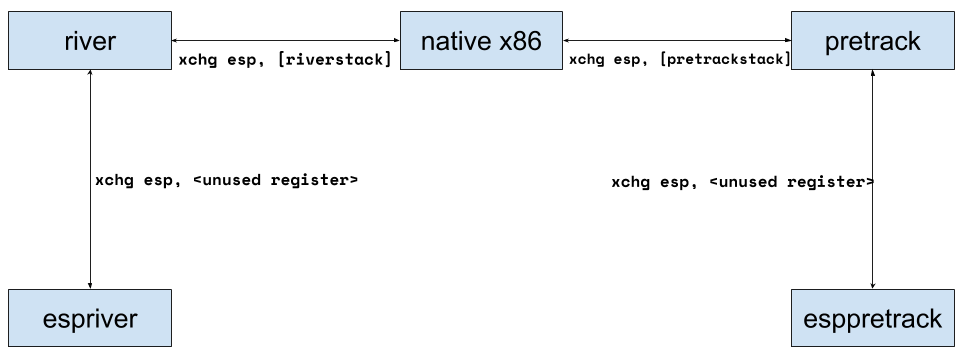
\includegraphics[width=\textwidth]{river-transition-handling}
	\label{img:river-transition-handling}
	\caption{River transition handling}
\end{figure}

\subsection{Assembling native instructions}
\label{ssec:assembling-native-instructions}
Most native instructions are assembled back to their original representations. The sole exceptions are branch instructions (jumps, conditional jumps, calls, returns, syscalls). Details will follow in future versions of this document.\\

\subsection{Assembling river instructions}
All river instructions are assembled directly to their binary counterpart.\\

\subsection{Assembling pretrack instructions}
Some pretrack instructions do not have a direct binary correspondent. See \autoref{table:assembling-pretrack-instructions}.\\
\begin{table}[h]
	\begin{tabular}{| l | l |}
		\hline
		\textbf{Instruction mnemonic} & \textbf{Native equivalent}\\ \hline
		pretrackpushf &	pushf\\ \hline
		pretrackpush reg & push reg\\ \hline
		\multirow{4}{*}{pretracklea mem} & mov [tmp], <unused_reg>\\
		& lea <unused_reg>, mem\\
		& push <unused_reg>\\
		& mov <unused_reg>, [tmp]\\ \hline
		pretrackpush mem & push mem\\ \hline
	\end{tabular}
	\caption{Pretrack transition table}
	\label{table:assembling-pretrack-instructions}
\end{table}

\chapter{Execution API}
\label{chapter:execution-api}
\textit{Note: The documentation in \autoref{chapter:execution-api} is subject to a lot of changes.}\\
While evaluating binary code the user regains control of the execution after each basic block. The user must implement the following callback in order to steer the program execution:
\lstinputlisting[language=C]{./code/BranchHandler.h}
\begin{table}[H]
	\begin{tabular}{| p{6cm} | p{10cm} |}
		\hline
		\textbf{Parameter name} & \textbf{Meaning}\\ \hline
		\multirow{2}{*}{pEnv} & An object encapsulating the entire execution environment. The user may store generic data under the pEnv->userContext field.\\
		& For allocating space for the userContext the user needs to call the AllocUserContext function.\\ \hline
		address & The address of the next instruction that will be executed (in case the execution goes forward.\\ \hline
	\end{tabular}
	\caption{Branch Handler Parameters}
\end{table}
The BranchHandler needs to return one of the two values in \autoref{table:branchhandler-return}.\\
\begin{table}[H]
	\begin{tabular}{| p{6cm} | p{10cm} |}
		\hline
		\textbf{Return value} & \textbf{Meaning}\\ \hline
		EVALUATE_FORWARD & Execution goes forward. The callback will be called after the next basic block is executed.\\ \hline
		EVALUATE_BACKWARD & All changes made by the last executed basic block are rolled back. The callback gets called after the rollback.\\ \hline
	\end{tabular}
	\label{table:branchhandler-return}
	\caption{Branch Handler Return Values}
\end{table}
If a basic block ends with a syscall the following callback is called:
\lstinputlisting[language=C]{./code/SysHandler.h}
This allows the user to globally save the machine state.\\
\begin{tabular}{| p{6cm} | p{10cm} |}
	\hline
	\textbf{Parameter name} & \textbf{Meaning}\\ \hline
	pEnv & An object encapsulating the entire execution environment. The user may store generic data under the pEnv->userContext field.\\ \hline
\end{tabular}

\appendix

\end{document}
